\documentclass[12pt,compress,aspectratio=169]{beamer}

\usetheme{metropolis}
\setbeamersize{text margin left=.5cm,text margin right=.5cm}
%  \addtobeamertemplate{background canvas}{\transfade}{}
\setbeamertemplate{navigation symbols}{} % suppress nav bar
%  \setbeamercovered{transparent}

%\usepackage[utf8]{inputenc}
\usefonttheme{professionalfonts}
%\usefonttheme[onlymath]{serif}
%\usepackage{unicode-math}
\usepackage{amsmath}
\usepackage{siunitx}
%\usepackage{graphicx}
\usepackage{tikz}
\usepackage{mathpazo}
%\usepackage{mathtools}
%\usepackage{unicode-math}
%\usepackage[scaled]{helvet}
\usepackage{bm}
%\usepackage{xcolor,colortbl}
%\usepackage{hyperref}

%\setsansfont{Lato-Regular}
%\setmathfont{Gentium}
\setmonofont{Ubuntu Mono}
\setlength{\parskip}{0pt}
\renewcommand{\baselinestretch}{1}

\sisetup{
  number-math-rm=\mathnormal,
  per-mode=symbol
}



\title{Topic 1: Introduction \& Kinematics}
\subtitle{Advanced Placement Physics}
\author[TML]{Dr.\ Timothy Leung}
\institute{Olympiads School}
\date{November 2, 2019}

\newcommand{\pic}[2]{\includegraphics[width=#1\textwidth]{#2}}
\newcommand{\mb}[1]{\ensuremath\mathbf{#1}}
\newcommand{\eq}[2]{\vspace{#1}{\Large\begin{displaymath}#2\end{displaymath}}}
\newcommand{\magdir}[2]{#1\text{ [#2]}}

\begin{document}

\begin{frame}{}

  {\LARGE
    \begin{center}
      \textbf{WELCOME TO AP PHYSICS}
    \end{center}
  }
\end{frame}


%\section{Housekeeping}

\begin{frame}{Pre-requisites}
  \begin{itemize}
  \item\textbf{Physics 11 and 12} %As AP Physics is primarily taught at the
    %first-year university level
    You will need to be comfortable with the topics covered in high-school
    level physics courses.
  \item\textbf{Calculus} The AP Physics C exams are calculus based, and you
    will be required to perform basic differentiation and integration. You
    don't need to be an expert, but basic knowledge is required.
    Differentiation and integration in the course are generally not
    difficult, but there are occasional challenges.
  \item\textbf{Vectors} You need to be comfortable with vector operations,
    including addition and subtraction, multiplication and division by
    constants, as well as dot products and cross products.
  \end{itemize}
\end{frame}



\begin{frame}{The AP Physics Exams}
  There are 4 AP Physics exams:
  \begin{itemize}
  \item Physics 1
  \item Physics 2
  \item Physics C--Mechanics
  \item Physics C--Electricity and Magnetism
  \end{itemize}
  Offered in first or second week of May of each year. The Physics C exams
  are calculus based; Physics 1 and 2 exams are algebra based.
\end{frame}



\begin{frame}{Classroom Rules}{Same as in Physics 11 and 12}
  \begin{itemize}
  \item Treat each other with respect
  \item Raise your hands if you have a question. Don't wait too long
  \item E-mail me at \texttt{tleung@olympiadsmail.ca} for any questions related
    to physics and math and engineering
  \item Do \textbf{\emph{not}} try to find me on social media
  \end{itemize}
\end{frame}


\begin{frame}
  \titlepage
\end{frame}

\begin{frame}{Files for You to Download}
  \begin{itemize}
  \item\texttt{PhysAP-courseOutline.pdf}--The course outline
  \item\texttt{PhysAP-equationSheet.pdf}--An equation sheet that you use during
    the exams
  \item\texttt{PhysAP-01-kinematics.pdf}--These presentation slides
  %\item\texttt{PhysAP-02-dynamics.pdf}--The presentation slides for the next
  %  topic
  \item\texttt{PhysAP-01-Homework.pdf}--Homework problems for Topic 1.
  \end{itemize}
  
  \vspace{.1in}Please download/print the PDF file for the class slides before
  each class. There is no point copying notes that are already on the slides.
  Instead, focus on things that aren't necessarily on the slides. If you wish
  to print the slides, we recommend printing 4 slides per page.
\end{frame}



\section{Vectors}

\begin{frame}{Notes on  Writing Vectors}
  In this course, vectors are \emph{printed} (e.g.\ on the slides) using a bold
  face font, while the ``arrow on top'' notation is used when \emph{writing}
  (e.g.\ on the blackboard)
  \vspace{.1in}
  \begin{columns}
    \column{.43\textwidth}
    \textbf{In print (books, journal papers)}
    \vspace{-.2in}{\LARGE
      \begin{displaymath}
        \mb{v}\quad\mb{F}_g\quad\mb{p}\quad\mb{I}
      \end{displaymath}
    }
    
    \column{.5\textwidth}
    \textbf{Handwritten (used by some books)}
    \vspace{-.2in}{\LARGE
      \begin{displaymath}
        \vec{v}\quad\vec{F}_g\quad\vec{p}\quad\vec{I}
      \end{displaymath}
    }
  \end{columns}
  Magnitude of vectors are expressed in one of two ways:
  \vspace{.1in}
  \begin{columns}
    \column{.5\textwidth}
    \textbf{With absolute-value sign}
    \vspace{-.2in}{\LARGE
      \begin{displaymath}
        |\mb{v}|\quad|\mb{F}_g|\quad|\mb{p}|\quad|\mb{I}|
      \end{displaymath}
    }
    \column{.42\textwidth}
    \textbf{Or as a scalar}
      \vspace{-.2in}{\LARGE
        \begin{displaymath}
          v\quad F_g\quad p \quad I
        \end{displaymath}
      }
  \end{columns}
\end{frame}


\begin{frame}{Writing Vectors}
  In Grades 11 and 12 Physics, vectors are usually written by separating the
  magnitude from the direction. For example, a velocity vector can be written
  as:
  
  \eq{-.2in}{
    \mb{v}=\SI{4.5}{\metre\per\second}\text{ [N $55^\circ$ E]}
  }
  
  \vspace{-.15in}This approach is based on using the
  \textbf{polar coordinate system}, which is the preferred coordinate system
  for circular motion. In general, polar coordinate system is
  \begin{itemize}
  \item Intuitive for describing \emph{one} vector in 2D
  \item Complicated when extended into 3D; need to extend to
    \textbf{spherical coordinate system} or the
    \textbf{cylindrical coordinate system}
  \item Difficult to perform vector arithmetic for \emph{rectilinear} motion
  \end{itemize}
\end{frame}


\begin{frame}{IJK Vector Notation}
  For rectilinear motion, vectors in 2D/3D Cartesian space are generally
  written in their $x$, $y$ \& $z$ components using the ``IJK notation'':

  \eq{-.2in}{
    \mb{A}=A_x\bm{\hat{\imath}} + A_y\bm{\hat{\jmath}} + A_z\bm{\hat{k}}
  }

  \vspace{-.2in}
  \begin{itemize}
  \item $\bm{\hat{\imath}}$, $\bm{\hat{\jmath}}$ and $\bm{\hat{k}}$ are
    \textbf{basis vectors} indicating the directions of the $x$, $y$ and $z$
    axes. Basis vectors are \textbf{unit vectors} (i.e.\ length $1$).
  \item The IJK notation does not give the magnitude of the vector, which needs
    to be calculated:

    \eq{-.25in}{
      A=|\mb{A}|=\sqrt{A_x^2 + A_y^2 + A_z^2}
    }
  \end{itemize}
\end{frame}


\begin{frame}{Vector Addition and Subtraction}
  Adding and subtracting vectors is straightforward:

  \eq{-.2in}{
    \mb{A}\pm\mb{B}=
    (A_x\pm B_x)\bm{\hat{\imath}} +
    (A_y\pm B_y)\bm{\hat{\jmath}} +
    (A_z\pm B_z)\bm{\hat{k}}
  }
\end{frame}


\begin{frame}{Dot Product}
  The vector \textbf{dot product} (inner product) is the scalar multiplication
  of two vectors. It is determined by the magnitude of the two vectors and the
  cosine of the angle between them:

  \eq{-.25in}{
    C=\mb{A}\cdot\mb{B}=\mb{B}\cdot\mb{A}=AB\cos\theta
  }
  \begin{itemize}
  \item\vspace{-.15in}You have been using this in the calculation of mechanical
    work
  \item $C$ is the \emph{projection} of the vector $\mb{A}$ onto $\mb{B}$, or
    the component of $\mb{A}$ along $\mb{B}$
  \item $\bm{\hat{\imath}}\cdot\bm{\hat{\imath}}=1$,
    $\bm{\hat{\jmath}}\cdot\bm{\hat{\jmath}}=1$, and
    $\bm{\hat{k}}\cdot\bm{\hat{k}}=1$
  \item For vectors written in IJK notation, and the magnitude and direction
    of the vector is not immediately known:
    
    \eq{-.25in}{
      C=\mb{A}\cdot\mb{B}=A_xB_x+A_yB_y+A_zB_z
    }
  \end{itemize}
\end{frame}


\begin{frame}{Cross Products}
  \vspace{.2in}
  \begin{columns}
    \column{.75\textwidth}
    The vector \textbf{cross product} is the vector multiplication of two
    vectors:

    \eq{-.25in}{
      \mb{C}=\mb{A}\times\mb{B}
    }
    \begin{itemize}
    \item\vspace{-.15in}The magnitude of the cross product is determined by the
      magnitude of $\mb{A}$ and $\mb{B}$ and the angle $\theta$ between them:

      \eq{-.3in}{
        C=AB\sin\theta
      }
    \item $\mb{C}$ is perpendicular to both $\mb{A}$ and $\mb{B}$; its direction
      given by the right hand rule
    \item Used in extensively in rotational motion and in electromagnetism
    \end{itemize}

    \column{.25\textwidth}
    \pic{1}{cross-product.png}
  \end{columns}
\end{frame}


\begin{frame}{Cross Products}
  The cross product of any two vectors in 3D space is the determinant of this
  $3\times 3$ matrix:
  
  \eq{-.2in}{
    \mb{A}\times\mb{B}=
    \left|
    \begin{matrix}
      \bm{\hat{\imath}} & \bm{\hat{\jmath}} & \bm{\hat{k}}\\
      A_x & A_y & A_z\\
      B_x & B_y & B_z
    \end{matrix}
    \right|
%      &=(A_yB_z-A_zB_y)\bm{\hat{\imath}} +
%      (A_zB_x-A_xB_z)\bm{\hat{\jmath}} +
%      (A_zB_y-B_yA_x)\bm{\hat{k}}
  }
  
  The order of the cross product is important. (This is why you
  have to get the right hand rule correctly.)

  \eq{-.3in}{
    \mb{A}\times\mb{B}=-\mb{B}\times\mb{A}
  }
\end{frame}


\begin{frame}{Cross Product}
  Most cross products applications in AP Physics are simpler, so we
  only have to remember this circle:
  \begin{center}
    \pic{.12}{cross-product-circle.png}
  \end{center}
  \begin{itemize}
  \item The direction of the arrow gives the index of the cross product
    (e.g.\ $\bm{\hat{\imath}}\times\bm{\hat{\jmath}}=\bm{\hat{k}}$)
  \item Going against the direction of the arrow gives the negative of the next
    index (e.g.\ $\bm{\hat{k}}\times\bm{\hat{\jmath}}=-\bm{\hat{\imath}}$)
  \end{itemize}
\end{frame}


\section{Calculus}

\begin{frame}{Calculus is Invented for Physics}{Thanks, Issac Newton}
  \begin{itemize}
  \item We cannot learn physics properly without calculus %(you got away with it
    %long enough in grades 11 and 12\ldots)
  \item Calculus was ``invented'' so that we can understand motion, especially
    non-constant velocities and accelerations
  \item You may have already noticed that a lot of the word problems in
    calculus are really physics problems
  \end{itemize}
\end{frame}


\begin{frame}{Differentiation and Integration}
  \begin{itemize}
  \item\textbf{Differential Calculus}
    \begin{itemize}
    \item How quickly something is changing (``rate of change'' of a quantity)
    \item Math: slopes of functions
    \item Physics: how quickly a physical quantity is changing in time and/or
      space
    \item Examples: velocity (how quickly position changes with time),
      acceleration (how quickly velocity changes with time), power (how quickly
      work is done), electric fields (how electric potential changes in space)
    \end{itemize}
  \item\textbf{Integral Calculus}
    \begin{itemize}
    \item The opposite of differentiation
    \item We use it to compute the area under a curve, or
    \item Summation of many small terms
    \item Examples: area under the $\mb{v}$-$t$ graph (displacement), area
      under the $\mb{F}$-$t$ graph (impulse), area under the $\mb{F}$-$d$ graph
      (work)
    \end{itemize}
  \end{itemize}
\end{frame}


\begin{frame}{Derivative}
  For any arbitrary function $f(x)$, the derivative with respect to
  (``w.r.t.'') $x$ is:

  \eq{-.2in}{
    \boxed{f'(x)=\lim_{h\rightarrow 0}\frac{f(x+h)-f(x)}{h}}
  }

  The ``limit as $h$ approaches $0$'' is the mathematical way of making $h$
  a very small non-zero number
\end{frame}



\begin{frame}{Know the Tricks for Differentiation}
  The derivative of a constant (``$C$'') w.r.t.\ any variable is zero.
  %(Obviously, the slope of any function $f(x)=C$ is zero.)

  \eq{-.2in}{
    \frac{dC}{dx}=0
  }
    
  \vspace{-.1in}A constant multiple of any function $f$ can be factored outside
  the derivative:
    
  \eq{-.2in}{ \frac{d}{dx}(af)=a\frac{df}{dx} }

  \vspace{-.1in}The derivative of a sum is the sum of a derivative:
  
  \eq{-.2in}{
    \frac{d}{dt}\left(f(t)+g(t)\right) = \frac{df}{dt}+\frac{dg}{dt}
  }
\end{frame}



\begin{frame}{Time-Saving Rules for Differentiation}
  Power Rule:

  \eq{-.2in}{
    \frac{d}{dt}\left(t^n\right) = nt^{n-1}%\quad\text{\normalsize for}
    %\quad n\neq 0
  }

  \vspace{-.1in}Product Rule:

  \eq{-.2in}{
    \frac{d}{dx}\left(f(x)g(x)\right)=f'(x)g(x)+f(x)g'(x)
  }
    
  \vspace{-.1in}Chain Rule:

  \eq{-.2in}{
    \frac{d}{dx}f\left(g(x)\right)=f'(g(x))g'(x)
  }
\end{frame}



\begin{frame}{Time-Saving Rules for Differentiation}
  Quotient Rule:

  \eq{-.2in}{
    \frac{d}{dx}\left[\frac{f(x)}{g(x)}\right]=
    \frac{f'(x)g(x)-g'(x)f(x)}{\left(g(x)\right)^2}
  }

  Thankfully you will probably never see this in a physics test in AP or
  first-year university
\end{frame}



\begin{frame}{Elementary Derivatives}
  Note how sines and cosines are related:
  
  \eq{-.2in}{
    \frac{d}{dt}\sin t = \cos t \quad\quad\quad
    \frac{d}{dt}\cos t = -\sin t
  }

  And the exponential function:
  
  \eq{-.2in}{
     \frac{d}{dt}e^{at} = ae^{at}
  }

  When studying \textbf{harmonic motion} and \textbf{circular motion},
  trigonometric functions and exponential are often used. We will also find out
  the relationship between complex exponential functions and sine/cosine
  functions.
\end{frame}



\begin{frame}{Partial Derivatives}
  Some functions have many variables (multi-variable function). For example,
  gravitational potential energy $U_g$ has three variables: masses $m_1$ and
  $m_2$ and the distance $r$ between them:

  \eq{-.2in}{
    U_g(m_1,m_2,r)=-\frac{Gm_1m_2}{r}
  }

  Differentiating w.r.t.\ one variable while holding others constant gives its
  \textbf{partial derivative}. (We use the $\partial$ symbol). e.g.\ the
  partial derivative of $U_g$ w.r.t.\ $r$ is

  \eq{-.2in}{
    \frac{\partial U_g}{\partial r}=\frac{Gm_1m_2}{r^2}
  }

  FYI: this is the relationship between $U_g$ and $\mb{F}_g$.
\end{frame}


\begin{frame}{Integration}
  If $F(x)$ is the anti-derivative of $f(x)$, they are related this way:
  
  \eq{-.15in}{
    \frac{d}{dx}F(x)=f(x)\quad\longrightarrow\quad F(x)=\int f(x)dx
  }
    
  The mathematical proof is the \textbf{fundamental theorem of calculus}.
\end{frame}



\begin{frame}{Common Integrals in Physics}
  Integration, while often necessary, can be very daunting, but integrals in AP
  Physics are generally straightforward. These rules should help in most cases:

  \begin{itemize}
  \item Power rule in reverse:

    \eq{-.2in}{ \int x^ndx=\frac{1}{n+1}x^{n+1}+C}

  \item Natural logarithm:

    \eq{-.3in}{ \int \frac{1}{x}dx =\ln |x|+C }
  \end{itemize}
\end{frame}


\begin{frame}{Common Integrals in Physics}
  \begin{itemize}
  \item Sines and cosines:
    
    \vspace{-.3in}{\Large
      \begin{align*}
        \int\cos xdx&=\sin x+C\\
        \int\sin xdx&=-\cos x+C
      \end{align*}
    }
  \end{itemize}
  %We can ``ignore'' (i.e.\ cancel) the constant of integration $C$ for definite
  %integrals.
\end{frame}


\begin{frame}{Definite vs.\ Indefinite Integral}{This Should Be a Review}
  \begin{itemize}
  \item Integrals can be either \textbf{indefinite} or \textbf{definite}
  \item An ``indefinite'' integral is another function, e.g.\ position
    $\mb{x}(t)$ as a function of time is found by integrating velocity
    $\mb{v}(t)$:

    \eq{-.2in}{
      \mb{x}(t)=\int\mb{v}(t)dt=\cdots+\mb{C}
    }
  \item A \textbf{constant of integration} $\mb{C}$ is added to the integral
    $\mb{x}(t)$. It is obtained through applying ``initial condition'' to the
    problem.
  \end{itemize}
\end{frame}


\begin{frame}{Definite Integrals}
  A \textbf{definite integral} has lower and upper bounds. e.g.\ given
  $\mb{v}(t)$, the displacement between $t_1$ and $t_2$ can be found:

  \eq{-.2in}{
    \Delta\mb{x}=\int_{t_0}^{t_1} \mb{v}(t)dt
  }

  Once we have computed the integral, we evaluate the limits:
  
  \eq{-.2in}{
    \Delta\mb{x} =
    \mb{x}(t)\Big|^{t_1}_{t_0}=
    \mb{x}(t_1)-\mb{x}(t_0)=
    \mb{x}_1-\mb{x}_0
  }

  The constant of integration $\mb{C}$ cancels when we evaluate the upper and
  lower bounds.
\end{frame}


\section{Kinematics}

\begin{frame}{Kinematics}
  \begin{itemize}
  \item\textbf{Kinematics} is a discipline with in mechanics for describing the
    motion of points, bodies (objects), and systems of  bodies (groups of
    objects)
  \item Relationship between 
    \begin{itemize}
    \item Position
    \item Displacement
    \item Distance 
    \item Velocity
    \item Speed
    \item Acceleration
    \end{itemize}
  \item Kinematics does not deal with what causes motion
  \end{itemize}
\end{frame}



\begin{frame}{Position}
  \textbf{Position} is a vector describing the location of an object in a
  coordinate system (usually \emph{Cartesian}; can also be \emph{polar},
  \emph{cylindrical} or \emph{spherical}). The origin of the coordinate system
  is called ``reference point''.

  \eq{-.2in}{
    \mb{x}(t)=x(t)\bm{\hat{\imath}} + y(t)\bm{\hat{\jmath}} + z(t)\bm{\hat{k}}
  }
  \begin{itemize}
  \item\vspace{-.15in}The SI unit for position is a \textbf{meter},
    \si{\metre}
  \item The components $x$, $y$ and $z$ are the coordinates along those axes
  \item The vector is a function of time $t$
  \end{itemize}
\end{frame}



\begin{frame}{Displacement}
  \textbf{Displacement} is the change in position from $1$ to $2$ within the
  same coordinate system:

  \eq{-.45in}{
      \Delta\mb{x}=\mb{x}_2-\mb{x}_1
      =(x_2-x_1)\bm{\hat{\imath}}+
      (y_2-y_1)\bm{\hat{\jmath}}+
      (z_2-z_1)\bm{\hat{k}}
  }
  \begin{itemize}
  \item IJK notation makes vector addition and subtraction less prone to errors
  \item Since reference point $\mb{x}_{\textrm{ref}}=\mb{0}$, the position
    $\mb{x}$ is also its displacement from the reference point
  \end{itemize}
\end{frame}


\begin{frame}{Distance}{Similar to Displacement}
  \begin{columns}
    \column{.7\textwidth}
    \textbf{Distance} $s$ is a quantity that is \emph{related} to displacement.
    \begin{itemize}
    \item The length of the path taken when an object moves from $\mb{d}_1$ to
      $\mb{d}_2$
    \item A scalar quantity
    \item Always positive, i.e.\ $s\geq 0$
    \item Although the magnitude of the displacement vector is also a scalar,
      it is not necessarily the same as distance
    \item In general, $s\geq |\Delta\mb{d}|$
    \end{itemize}
    
    \column{.3\textwidth}
    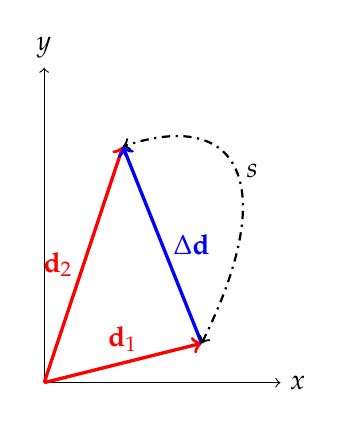
\begin{tikzpicture}[scale=.5]
      \draw[->](0,0)--(6,0) node[pos=1,right]{$x$};
      \draw[->](0,0)--(0,8) node[pos=1,above]{$y$};
      \draw[->,red,very thick] (0,0)--(4,1) node[midway,above]{$\mb{d}_1$};
      \draw[->,red,very thick] (0,0)--(2,6) node[midway,left]{$\mb{d}_2$};
      \draw[->,blue,very thick](4,1)--(2,6) node[midway,right]{$\Delta\mb{d}$};
      \draw[thick,dash dot,<->] (4,1)..controls (6,5) and (5,7)..(2,6)
      node[midway,right]{$s$};
    \end{tikzpicture}
  \end{columns}
\end{frame}



\begin{frame}{Instantaneous Velocity}
  \framesubtitle{Time Derivative of Position}
  If position $\mb{x}$ is a differentiable function in time $t$, then velocity
  $\mb{v}$ can be found at any time $t$. The \textbf{instantaneous velocity} of
  an object is the rate of change of its position vector w.r.t.\ time:

  \eq{-.2in}{
    \boxed{\mb{v}(t)= \frac{d\mb{x}(t)}{dt}}
  }
  
  Since $\mb{x}$ has $x$, $y$ and $z$ components in the
  $\bm{\hat{\imath}}$, $\bm{\hat{\jmath}}$ and $\bm{\hat{k}}$ directions that
  are linearly independent, we can take the derivative w.r.t.\ time in
  every component:

  \eq{-.3in}{
    \mb{v}(t)= \frac{d\mb{x}}{dt}=
    \frac{dx}{dt}\bm{\hat{\imath}} +
    \frac{dy}{dt}\bm{\hat{\jmath}} + \frac{dz}{dt}\bm{\hat{k}}=
    v_x\bm{\hat{\imath}} + v_y\bm{\hat{\jmath}} + v_z\bm{\hat{k}}
  }
\end{frame}


\begin{frame}{Integrating Velocity to Get Position/Displacement}
  If instantaneous velocity $\mb{v}$ is the rate of change of position
  $\mb{x}$ w.r.t. time $t$, then $\mb{x}$ is the time integral of $\mb{v}$:
  
  \eq{-.2in}{
    \mb{x}(t)=\int\mb{v}(t)dt + \mb{x}_0
  }
  
  The constant of integration $\mb{x}_0=\mb{x}(0)$ is the
  \emph{initial position} at $t=0$. As both $\mb{x}$ and $\mb{v}$ are vectors,
  we integrate each component to get $\mb{x}$:

 \eq{-.2in}{ \mb{x}(t)= \left(
    \int v_x\bm{\hat{\imath}} +
    \int v_y\bm{\hat{\jmath}} +
    \int v_z\bm{\hat{k}}
    \right) dt + \mb{x}_0
  }
\end{frame}


\begin{frame}{Average Velocity}
  The \textbf{average velocity} of an object is the change in position
  $\Delta\mb{x}$ over a finite time interval $\Delta t$:

  \eq{-.3in}{
    \boxed{\overline{\mb{v}}= \frac{\Delta\mb{x}}{\Delta t}}
  }
  
  Like instantaneous velocity, we can find the $x$, $y$ and $z$ components of
  average velocity by separating components in each direction:

  \eq{-.2in}{
    \overline{\mb{v}}=
    \frac{\Delta x}{\Delta t}\bm{\hat{\imath}} +
    \frac{\Delta y}{\Delta t}\bm{\hat{\jmath}} +
    \frac{\Delta z}{\Delta t}\bm{\hat{k}}
  }
\end{frame}



\begin{frame}{Instantaneous Speed}
  \textbf{Intantaneous speed} the rate of change of \emph{distance} w.r.t.\
  time:

  \eq{-.2in}{
    \boxed{
      v=\frac{ds}{dt}
    }
  }
  \begin{itemize}
  \item Since distance of any path must always be positive $s>0$, instantaneous
    speed must also be positive
  \item Instantaneous speed $v$ is the magnitude of the instantaneous velocity
    vector $\mb{v}$
  \end{itemize}
\end{frame}



\begin{frame}{Average Speed}
  Likewise, \textbf{average speed} is similar to average velocity: it is the
  distance travelled over a finite time interval.
  
  \eq{-.2in}{
    \boxed{
      \overline{v}=\frac{s}{\Delta t}
    }
  }

%  \begin{itemize}
%
%  \end{itemize}
\end{frame}



\begin{frame}{Path}
  Sometimes instead of explicitly describing the position $x=x(t)$ and $y=y(t)$,
  the path of an object can be given in terms of $x$ coordinate $y=y(x)$, while
  giving the $x$ (or $y$) coordinate as a function of time.
  \begin{itemize}
  \item In this case, substitute the expression for $x(t)$ into $y=y(x)$ to
    get an expression of $y=y(t)$
  \item Take derivative using chain rule to get $v_y=v_y(t)$
  \end{itemize}
\end{frame}


\begin{frame}{Instantaneous Acceleration}
  In the same way that velocity is the rate of change in position w.r.t.\ time,
  \textbf{acceleration} is the rate of change in velocity w.r.t.\ time:

  \eq{-.2in}{
    \boxed{\mb{a}(t)= \frac{d\mb{v}(t)}{dt}=\frac{d^2\mb{x}(t)}{dt^2}}
  }
  
  Acceleration is the second derivative of position, i.e.
  \begin{enumerate}
  \item Take derivative of $\mb{x}(t)$ to get $\mb{v}(t)=\mb{x}'(t)$
  \item Take derivative again of $\mb{v}(t)$ to get $\mb{a}(t)=\mb{v}'(t)$
  \end{enumerate}
\end{frame}



\begin{frame}{Special Notation When Differentiating With Time}
  Physicists and engineers use a special notation when the derivative is
  taken w.r.t.\ \emph{time}, by writing a dot above the variable:
  \begin{itemize}
  \item Velocity:

    \eq{-.35in}{
      \boxed{\mb{v}(t)= \dot{\mb{x}}}
    }
  \item Acceleration:

    \eq{-.35in}{
      \boxed{\mb{a}(t)= \dot{\mb{v}}=\ddot{\mb{x}}}
    }
  \end{itemize}

  We will use this notation whenever it is convenient
\end{frame}


\begin{frame}{Integrating Acceleration to Get Velocity}
  Velocity $\mb{v}(t)$ is the time integral of acceleration $\mb{a}(t)$:
    
  \eq{-.2in}{
    \mb{v}(t)=\int\mb{a}(t)dt+\mb{v}_0
  }

  Again, since both $\mb{v}$ and $\mb{a}$ are vectors, we need
  to integrate in each direction:

  \eq{-.2in}{
    \mb{v}(t)=
    \left(\int a_x\bm{\hat{\imath}} +
    \int a_y\bm{\hat{\jmath}} +
    \int a_z\bm{\hat{k}}\right) dt +\mb{v}_0
  }
\end{frame}


\begin{frame}{For Those Who Are Curious}
  The time derivative of acceleration is called \textbf{jerk}, with a unit
  of \si{\metre\per\second^3}:

  \eq{-.2in}{
    \mb{j}=\frac{d\mb{a}}{dt}=\frac{d^2\mb{v}}{dt^2}=\frac{d^3\mb{x}}{dt^3}
  }

  The time derivative of jerk is \textbf{jounce}, or \textbf{snap}, with a
  unit of \si{\metre\per\second^4}:
  
  \eq{-.2in}{
    \mb{s}=\frac{d\mb{j}}{dt}=\frac{d^2\mb{a}}{dt^2}=\frac{d^3\mb{v}}{dt^3}
    =\frac{d^4\mb{x}}{dt^4}
  }
  
  The next two derivatives of snap is facetiously called \textbf{crackle} and
  \textbf{pop}, but these higher derivatives of position vector are rarely seen.
  We will not be using these in AP Physics.
\end{frame}


\section{Motion Graphs}

\begin{frame}{Motion Graphs}
  For 1D motion, we can describe motion graphically using motion graphs, by
  plotting
  \begin{itemize}
  \item Position vs.\ time ($x-t$) graph
  \item Velocity vs.\ time ($v-t$) graph
  \item Acceleration vs.\ time ($a-t$) graph
  \end{itemize}
\end{frame}



\begin{frame}{Uniform Motion}
  \begin{center}
    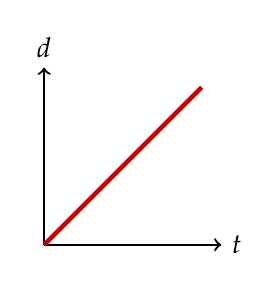
\begin{tikzpicture}[scale=.5]
      \draw[->,thick] (0,0)--(4.5,0) node[pos=1,right]{$t$};
      \draw[->,thick] (0,0)--(0,4.5) node[pos=1,above]{$d$};
      \draw[red!80!black,ultra thick](0,0)--(4,4);
    \end{tikzpicture}
    \hspace{.15in}
    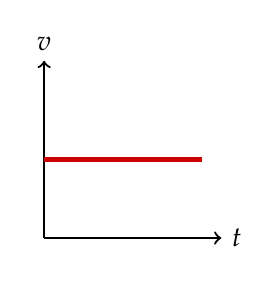
\begin{tikzpicture}[scale=.5]
      \draw[->,thick] (0,0)--(4.5,0) node[pos=1,right]{$t$};
      \draw[->,thick] (0,0)--(0,4.5) node[pos=1,above]{$v$};
      \draw[red!80!black,ultra thick](0,2)--(4,2);
    \end{tikzpicture}
    \hspace{.15in}
    \begin{tikzpicture}[scale=.5]
      \draw[->,thick] (0,0)--(4.5,0) node[pos=1,right]{$t$};
      \draw[->,thick] (0,0)--(0,4.5) node[pos=1,above]{$a$};
      \draw[red!80!black,ultra thick](0,0)--(4,0);
    \end{tikzpicture}
  \end{center}
  \begin{itemize}
  \item Constant velocity has a straight line in the $d-t$ graph
  \item The slope of the $d-t$ graph is the velocity $v$
  \item The slope of the $v-t$ graph is the acceleration $a$, which is zero in
    this case
  \end{itemize}
\end{frame}


\begin{frame}{Uniform Acceleration}
  \begin{center}
    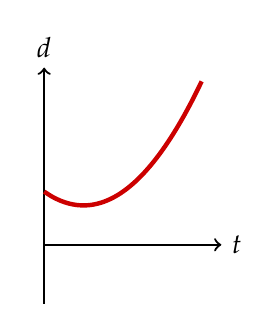
\begin{tikzpicture}[scale=.5]
      \draw[->,thick] (0,0)--(4.5,0) node[pos=1,right]{$t$};
      \draw[->,thick] (0,-1.5)--(0,4.5) node[pos=1,above]{$d$};
      \draw[smooth,samples=20,domain=0:4,red!80!black,ultra thick]
      plot({\x},{0.35*(\x-1)*(\x-1)+1});
    \end{tikzpicture}
    \hspace{.15in}
    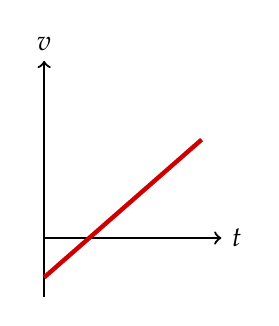
\begin{tikzpicture}[scale=.5]
      \draw[->,thick] (0,0)--(4.5,0) node[pos=1,right]{$t$};
      \draw[->,thick] (0,-1.5)--(0,4.5) node[pos=1,above]{$v$};
      \draw[red!80!black,ultra thick](0,-1)--(4,2.5);
    \end{tikzpicture}
    \hspace{.15in}
    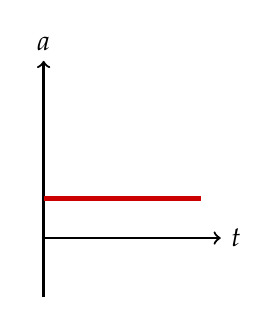
\begin{tikzpicture}[scale=.5]
      \draw[->,thick] (0,0)--(4.5,0) node[pos=1,right]{$t$};
      \draw[->,thick] (0,-1.5)--(0,4.5) node[pos=1,above]{$a$};
      \draw[red!80!black,ultra thick](0,1)--(4,1);
    \end{tikzpicture}
  \end{center}
  \begin{itemize}
  \item The $d-t$ graph for motion with constant acceleration is part of a
    \emph{parabola}
    \begin{itemize}
    \item If the parabola is \emph{convex}, then acceleration is positive
    \item If the parabola is \emph{concave}, then acceleration is negative
    \end{itemize}
  \item The $v-t$ graph is a straight line; its slope (a constant) is the
    acceleration
  \end{itemize}
\end{frame}


\begin{frame}{Simple Harmonic Motion}
  For oscillatory motion, or \textbf{harmonic motion}, neither position,
  velocity nor acceleration are constant:

  \vspace{-.1in}
  \begin{center}
    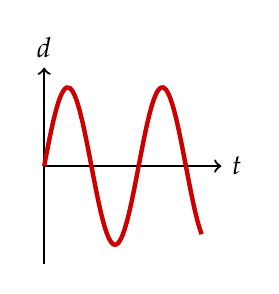
\begin{tikzpicture}[scale=.5]
      \draw[->,thick] (0,0)--(4.5,0) node[pos=1,right]{$t$};
      \draw[->,thick] (0,-2.5)--(0,2.5) node[pos=1,above]{$d$};
      \draw[smooth,samples=50,domain=0:4,red!80!black,ultra thick]
      plot({\x},{2*sin(150*\x)});
    \end{tikzpicture}
    \hspace{.15in}
    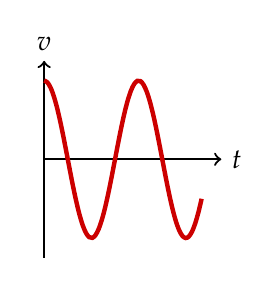
\begin{tikzpicture}[scale=.5]
      \draw[->,thick] (0,0)--(4.5,0) node[pos=1,right]{$t$};
      \draw[->,thick] (0,-2.5)--(0,2.5) node[pos=1,above]{$v$};
      \draw[smooth,samples=50,domain=0:4,red!80!black,ultra thick]
      plot({\x},{2*cos(150*\x)});
    \end{tikzpicture}
    \hspace{.15in}
    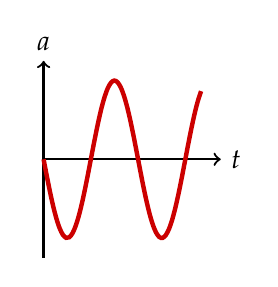
\begin{tikzpicture}[scale=.5]
      \draw[->,thick] (0,0)--(4.5,0) node[pos=1,right]{$t$};
      \draw[->,thick] (0,-2.5)--(0,2.5) node[pos=1,above]{$a$};
      \draw[smooth,samples=50,domain=0:4,red!80!black,ultra thick]
      plot({\x},{-2*sin(150*\x)});
    \end{tikzpicture}
  \end{center}
  Bottom line: regardless of the type motion,
  \begin{itemize}
  \item The $v-t$ graph is the slope of the $d-t$ graph
  \item The $a-t$ graph is the slope of the $v-t$ graph
  \end{itemize}
\end{frame}


\begin{frame}{Area Under $v-t$ Graph}
  The area under the $v-t$ graph is the displacement $x-x_0$. (This should be
  obvious, since $x$ is the time integral of $v$.)
  \begin{columns}
    \column{.3\textwidth}
    \begin{center}
      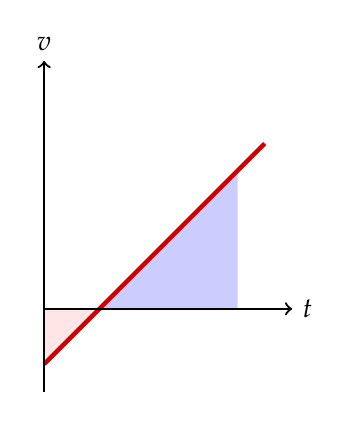
\begin{tikzpicture}[scale=.7]
        \draw[pink!40,fill=pink!40](0,0)--(0,-1)--(1,0)--cycle;
        \draw[blue!20,fill=blue!20](1,0)--(3.5,0)--(3.5,2.5)--cycle;
        \draw[red!80!black,ultra thick](0,-1)--(4,3);
        \draw[->,thick] (0,0)--(4.5,0) node[pos=1,right]{$t$};
        \draw[->,thick] (0,-1.5)--(0,4.5) node[pos=1,above]{$v$};
      \end{tikzpicture}
    \end{center}
    
    \column{.7\textwidth}
    \begin{itemize}
    \item If the area is \textcolor{red!40}{\emph{below}} the $x$ (time) axis,
      then the displacement is negative;
    \item If the area is \textcolor{blue!20}{\emph{above}} the time axis, then
      displacement is positive
    \end{itemize}
  \end{columns}
\end{frame}



\section{Kinematic Equations}

\begin{frame}{Kinematic Equations For Constant Acceleration}
  Although kinematic problems in AP Physics often require calculus, these basic
  kinematic equations are still a very powerful tool.
  \begin{columns}
    \column{.45\textwidth}

    \vspace{-.3in}{\Large
      \begin{align*}
        \mb{x} &= \mb{x}_0+ \mb{v}_0t + \frac{1}{2}\mb{a}t^2\\
        \mb{v} &=\mb{v}_0+\mb{a}t\\
        v^2 &= v_0^2+ 2a(x-x_0)
      \end{align*}
    }
    
    \column{.55\textwidth}
    \begin{itemize}
    \item The variables of interests are:

      \eq{-.4in}{
        \mb{x}_0\quad\mb{x}\quad\mb{v}_0 \quad\mb{v}\quad t\quad\mb{a}
      }
    \item Only applicable for constant acceleration
    \end{itemize}
  \end{columns}

  You will still encounter situations where integration is necessary.
\end{frame}


%\begin{frame}{Solving Typical Kinematics Problems}
%  
%  \textbf{One object:} the problem provides $3$ of the $5$ variables, and you
%  are asked to find a $4$th one.
%  \begin{itemize}
%  \item Define the positive direction (usually very obvious)
%  \item Apply the correct kinematic equation and solve the problem!
%  \end{itemize}
%
%  \vspace{.2in}\textbf{Two objects:} two objects are in motion. Usually one of
%  them is moving at constant velocity while the other is accelerating.
%  \begin{itemize}
%  \item Time interval $\Delta t$ and displacement $\Delta\mb{x}$ of the two
%    objects are related
%  \item Examples:
%    \begin{itemize}
%    \item Police car chasing a speeder
%    \item Two football players running towards each other
%    \item A person trying to catch the bus
%    \end{itemize}
%  \end{itemize}
%\end{frame}


\section{Projectile Motion}

\begin{frame}{Projectile Motion}
  \begin{itemize}
  \item For 2D problems, resolve the problem into its
    horizontal ($x$) and vertical ($y$) directions, and apply kinematic
    equations independently
  \item For projectile motion, there is no acceleration in the $x$ direction,
    i.e.\ $a_x=0$, therefore the kinematic equations reduce to just
    
    \eq{-.25in}{x=v_xt\bm{\hat{\imath}}}
  \item The only acceleration is in the $\bm{\hat{\jmath}}$ direction. In the
    standard Cartesian coordinate system, this usually means that
    $\bm{\hat{\jmath}}$ direction is \emph{up}:
    
    \eq{-.25in}{a_y=-g\bm{\hat{\jmath}}}
  \item The variable that connects the two directions is time $t$
  \end{itemize}
\end{frame}


\begin{frame}{Symmetric Trajectory}
  Trajectory is symmetric if the object lands at the same height as when it
  started. The angle $\theta$ is measured \emph{above the the horizontal}.
  \begin{itemize}
  \item Time of flight
    \eq{-.1in}{t_\mathrm{max}=\frac{2v_i\sin\theta}{g}}
  \item Range
    \eq{-.1in}{R=\frac{v_i^2\sin(2\theta)}{g}}
  \item Maximum height
    \eq{-.1in}{h_\mathrm{max}=\frac{v_i^2\sin^2\theta}{2g}}
  \end{itemize}
\end{frame}



\begin{frame}{Maximum Range}
  \eq{-.1in}{R=\frac{v_i^2\sin(2\theta)}{g}}
  
  \begin{itemize}
  \item For a given initial speed $v_i$, maximum range occurs at
    $\theta=45^\circ$
  \item For a given initial speed $v_i$ and range $R$, I can find a launch
    angle $\theta$ that gives the required range:
    
    \eq{-.2in}{
      \theta_1=\frac{1}{2}\sin^{-1}\left(\frac{Rg}{v_i^2}\right)
    }
  \item But there is another angle that \emph{gives the same range}!

    \eq{-.2in}{
      \theta_2=90^\circ-\theta_1
    }
  \end{itemize}
\end{frame}


\section{Relative Motion}

%\begin{frame}{Relative Motion}
%  Reconciling different frame of reference from different observer's
%  perspectives
%  \begin{columns} 
%    \column{.5\textwidth}
%    Example: sailing
%      \begin{itemize}
%      \item Account for current
%      \item Account for wind
%      %\item Account for man power on the boat
%      \end{itemize}
%      
%      \column{.5\textwidth}
%      \pic{1}{images/MJ_Newsletter_16-4-09_Rescue.jpg}
%  \end{columns}
%\end{frame}



\begin{frame}{Relative Motion}{Notation}
  When expressing relative motion, the first subscript ($A$) represents the
  moving object, and the second subscript ($B$) represents the frame of
  reference:

  \eq{-.4in}{
    \mb{v}_{AB}
  } 

  \vspace{-.15in}If an airplane (``P'') is traveling at
  \magdir{\SI{251}{\kilo\metre\per\hour}}{N} relative to Earth (``E''), its
  velocity is expressed as:

  \eq{-.4in}{
    \mb{v}_{PE}=\magdir{\SI{251}{\kilo\metre\per\hour}}{N}
  }
\end{frame}



\begin{frame}{Relative Motion}
  If the airplane flies in windy air (``A'') we must consider the velocity of
  the airplane relative to air $\mb{v}_{PA}$ and the velocity of the air
  relative to Earth $\mb{v}_{AE}$. The velocity of the airplane relative to
  Earth is therefore

  \eq{-.2in}{
    \mb{v}_{PE}=\mb{v}_{PA}+\mb{v}_{AE}
  }

  \vspace{-.1in}If an airplane is flying at a constant velocity of
  \magdir{\SI{253}{km/h}}{S} relative to the air and the air velocity is
  \magdir{\SI{24}{km/h}}{N}, what is the velocity of the airplane relative to
  Earth?
\end{frame}



\begin{frame}{Relative Motion}
  In classical mechanics, the equation for relative motion follows the
  \textbf{Galilean velocity addition rule}\footnote{This equation was
    thought to be so obvious that no one bother to give it a name until Einstein
    proved that it was incorrect for speeds close to the speed of light}:

  \eq{-.25in}{
    \boxed{\mb{v}_{AC}=\mb{v}_{AB}+\mb{v}_{BC}}
  }

  \vspace{-.15in}The velocity of $A$ relative to reference frame $C$ is the
  velocity of $A$ relative to reference frame $B$, plus the velocity of $B$
  relative to $C$.

  \vspace{.1in}If we add another frame of reference (``$D$''), the equation
  becomes:

  \eq{-.25in}{
    \mb{v}_{AD}=\mb{v}_{AB}+\mb{v}_{BC}+\mb{v}_{CD}
  }
\end{frame}


\begin{frame}{Typical Problems}
  For both AP Physics 1 and AP Physics C exams, questions involving kinematics
  usually appear in the multiple-choice section. The problems themselves are
  not very different compared to the Grade 12 Physics problems, but:
  \begin{itemize}
  \item You have to solve problems faster because of time constraint
  \item You can use $g=\SI{10}{m/s^2}$ to make your lives simpler
  \item A lot of problems are \emph{symbolic}, which means that they deal with
    the equations, not actual numbers
  \item Will be coupled with other types (e.g.\ dynamics and rotational) in
    the free-response section
  \item You \emph{will} be given an equation sheet
  \end{itemize}
\end{frame}

\end{document}
